
\subsection{Норменные группы}

		Пусть $L/K$~--- расширение Галуа локального поля $K$ с группой Галуа $G$. 

		\begin{definition} 
			Подгруппа группы $K^*$  называется \emph{норменной}, если существует такое конечное абелево расширение\footnote{т.е. расширение Галуа с абелевой группой Галуа} $L/K$ , что эта подгруппа в точности совпадает с $N_{L/K}L^*$.
		\end{definition}

	Рассмотрим  два абелевых расширения $L_1$ и $L_2$ локального поля $K$ и их композит: 

		\begin{center}
				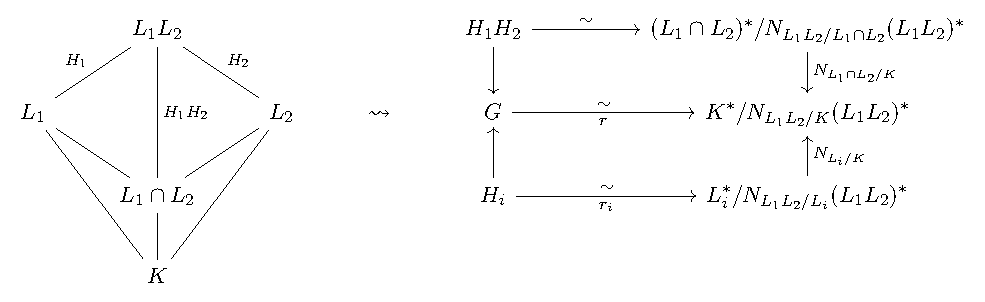
\includegraphics{lectures/6/pictures/cd_40.pdf}
	\end{center}

	По следствию~\ref{normal_subgroup_abelinisation} в  правой диаграмме горизонтальные стрелки~--- изоморфизмы.  Тогда из коммутативности мы получаем, что 
	\[
		r(H_1 H_2) = r(H_1)r(H_2) = N_{L_1/K}(L_1^*/N_{L_1 L_2/L_1}(L_1 L_2)^*) \cdot N_{L_2/K}(L_2^*/N_{L_1 L_2/L_1}(L_1 L_2)^*) = \frac{N_{L_1/K} L_{1}^*  \ \cdot \ N_{L_2/K}L_{2}^*}{N_{L_1L_2/K}(L_1 L_2)^*}
	\]
	С другой стороны, мы имеем 
	\[
		r(H_1 H_2) = \frac{N_{L_1 \cap L_2/K} (L_1 \cap L_2)^*}{ N_{L_1 L_2/K}(L_1 L_2)^*},
	\]
	а тогда мы имеем равенство 
	\[
		N_{L_1 \cap L_2/K} (L_1 \cap L_2)^* = N_{L_1/K}L_1^* \cdot N_{L_2/K}L_2^*.
	\]

	С другой стороны, мы знаем, что $H_1 \cap H_2 = 1$. Тогда 
	\[
		\frac{N_{L_1 L_2/K}(L_1 L_2)^*}{N_{L_1 L_2/K}(L_1 L_2)^*} = r(1) = r(H_1 \cap H_2) = r(H_1) \cap r(H_2) = \frac{ N_{L_1/K} L_1^* \cap N_{L_2/K} L_2^*}{N_{L_1 L_2/K}(L_1 L_2)^*},
	\]
	откуда мы получаем равенство 
	\[
		N_{L_1 L_2/K}(L_1 L_2)^* = N_{L_1/K}L_1^* \cap N_{L_2/K} L_2^*.
	\]
	Таким образом, мы показали, что пересечение и объединение норменных подгрупп~--- норменная подгруппа. 

	Что же можно сказать относительно включений? Из общей теории полей следует, что 
	\[
		L_1 \subset L_2 \implies N_{L_2/K} L_2^* \subset N_{L_1/K}L_1^*.
	\]
	Оказывается, есть и стрелочка в обратную сторону. Её мы также получим из равенств выше. Действительно, предположим, что $N_{L_2/K}L_2^* \supset N_{L_1/K} L_1^*$, тогда 
	\[
		N_{L_1 L_2/K}(L_1 L_2)^* = N_{L_2/K}L_2^*,
	\]
	а отсюда мы имеем 
	\[
		\Gal(L_1 L_2/K) \cong K^*/N_{L_1 L_2/K}(L_1L_2)^* = K^*/N_{L_2/K}L_2^* \cong \Gal(L_2/K).
	\]
	Но из такого равенства групп Галуа следует, что $L_1 L_2 = L_2 \Leftrightarrow L_1 \subset L_2$, что и требовалось.

	\begin{exercise}
		Если $N_{L/K}L^* \subset S \subset K^*$, то $S$~--- норменная подгруппа. 		 
	\end{exercise}
        \begin{proof}
		Применим соответствие Галуа. Действительно, рассмотрим $\theta_{L/K}\colon K^{*} \to K^*/N_{L/K}L^* \cong \Gal(L/K)$. Рассмотрим $\theta_L/K(S)$ и поле $F = L^{\theta_L/K(S)}$. Тогда имеет место такая коммутативная диаграмма: 
		\begin{center}
			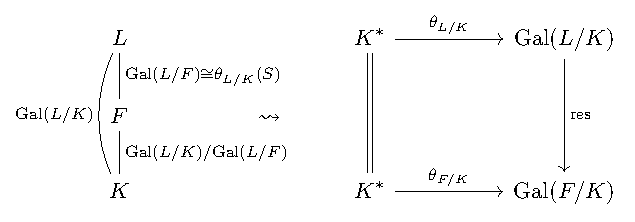
\includegraphics{lectures/6/pictures/cd_51.pdf}
		\end{center}
		Ну и из соответствия Галуа мы знаем, что 
		\[
			\theta_L/K(S) = \Ker\lr*{\Gal(L/K) \to \Gal(L/K)/\Gal(L/F) = \Gal(F/K)} \cong \Gal(L/F).
		\]
		Но тогда мы получаем, что 
		\[
			S = \theta_{L/K}^{-1}(\Gal(L/F)) = N_{F/K}F^*. 
		\]
	\end{proof}

	\begin{theorem} 
		Пусть $L/K$~--- конечное сепарабельное\footnote{это ограничение не по существу, но так доказывать проще (да и работаем мы в характеристике 0)} расширение\footnote{не обязательно Галуа!}. Тогда $N_{L/K}L^*$ является норменной группой. 
	\end{theorem}

	\begin{proof}
		Картинка у нас выглядит вот так: 

		где $E$~--- какое-то расширение Галуа поля $K$, содержащее $L$ в качестве подрасширения, а $F/K$~--- максимальное абелево расширение $K$, содержащееся в $L$.

		\begin{center}
				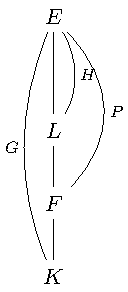
\includegraphics{lectures/6/pictures/cd_41.pdf}
	\end{center}

	Докажем, что $P = H [G, G] = H G'$. Действительно, из диаграммы мы видим, что $G/P$ абелева (так как это группа Галуа расширения $F/K$), откуда $G' \subset P \implies H G' \subset P$. Теперь применим соответствие Галуа: 
	\[
		H G' \leftrightarrow L \cap K_{ab},
	\]
	где $K_{ab}$~--- максимальное абелево расширение $K$, содержащееся в $E$. Но тогда $F = L \cap K_{ab}$ (просто по определению), тогда, так как соответствие Галуа~--- антиэквивалентность решеток, $P = H G'$. 

	Теперь рассмотрим такую коммутативную диаграмму: 
	\begin{center}
				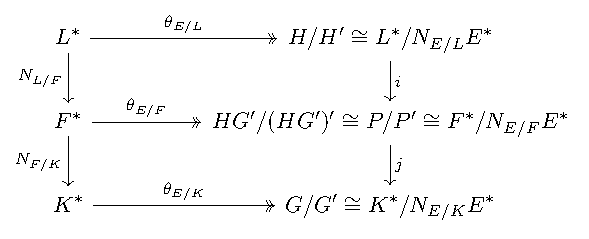
\includegraphics{lectures/6/pictures/cd_42.pdf}
	\end{center}

	где $\theta_{E/L}$~--- это сюръективное сквозное отображение 
	\[
		L^* \to L^*/N_{E/L}E^* \cong H/H'.
	\]
	Мы докажем, что $N_{L/K}L^* = N_{F/K}F^*$. Включение слева направо очевидно, а вот обратное включение~--- совсем не очевидно. Возьмём $x \in F^*$ и пройдёмся по верхнему коммутативному квадрату 
	\[
		\theta_{E/F}(x) = i \theta_{E/L}(y) \cdot \theta_{E/F}(u), \ \theta_{E/F}(u) \in G' / (HG')'.
	\]
	Значит, при факторизации по $G'$ этот элемент уйдёт в 0, то есть $j\theta_{E/F}(u) = 0$, что говорит нам, что если пройти в другом направлении, тоже получится 0, то есть
	\[
		\theta_{E/K}\lr*{N_{F/K}{u}} = 0 \implies N_{F/K}{u} \in N_{E/K}E^*.
	\]

	Значит, для некоторого $v$ мы имеем $N_{F/K}{u} = N_{E/K}{v}$. Продолжим диаграммный поиск, а именно, вновь пройдём по верхнему квадрату двумя способами: 

	\[
		\theta_{E/F}(x) = i \theta_{E/L}(y) \cdot \theta_{E/F}(u) \implies \theta_{E/F}(xu^{-1}) = i\theta_{E/L}(y) = \theta_{E/F}\lr*{N_{L/F}y} 
	\]
	Отсюда мы имеем, что 
	\[
		\theta_{E/F}(x u^{-1} (N_{L/F}y)^{-1}) = 1 \implies x u^{-1} (N_{L/F}y)^{-1}  = x u^{-1} N_{L/F}(y)^{-1} \in N_{E/F} E^*
	\]
	Применим к этому равенству $N_{F/K}$ и воспользуемся тем, что $N_{L/K} = N_{F/K} N_{L/F}$, а также $N_{E/K} = N_{F/K} N_{E/F}$, получим 
	\[
		N_{F/K}{x} \cdot N_{F/K}{u^{-1}} \cdot N_{L/K}{y^{-1}} \in N_{E/K}E^*
	\]

	Теперь вспомним, что в самой первой выкладке мы поняли, что $N_{F/K}{u^{-1}} = N_{E/K}{v^{-1}}$, что даёт нам 
	\[
				N_{F/K}{x} \cdot N_{E/K}{v^{-1}} \cdot N_{L/K}{y^{-1}} \in N_{E/K}E^*, 
	\]
	откуда мы имеем 

	\[
		N_{F/K}{x} \cdot N_{L/K}{y^{-1}} \in N_{E/K}E^*, 
	\]
	откуда мы заключаем, что $N_{F/K}{x} \in N_{L/K}L^*$, что и требовалось. 
	

	\end{proof}

    \subsection{Теория Куммера}

	Пусть у нас некоторая подгруппа $A \subset K^*$ индекса $m$, то есть $|K^*/A| = m$. В таком случае $K^{* m} \subset A$. Тогда для того чтобы доказать, что $A$~--- норменная, достаточно показать, что $K^{* m}$~--- норменная. 

	Докажем это в случае поля $K$ характеристики нуль. Сначала сделаем это в предположении $\zeta_m \in K$ (позже мы избавимся от этого предположения). 


	Пусть $\Bbbk$~--- поле, $m \ge 2$~--- целое число, $\Char{\Bbbk} \not \ \mid m$ и $\zeta_m \in \Bbbk$. 

	Рассмотрим $B$ такое, что $\Bbbk^{* m} \subset B \subset \Bbbk^{*}$ и $|B/\Bbbk^{* m}|$. Через $\Bbbk\lr*{\sqrt[m]{B}}$ мы будем обозначать композит всех расширений $\Bbbk\lr*{\sqrt[m]{b}}$ по $b \in B$. 

	\begin{theorem}[Куммер] 
		Расширение $\Bbbk\lr*{\sqrt[m]{B}}/\Bbbk$ конечно и $[\Bbbk\lr*{\sqrt[m]{B}} : \Bbbk] = |B/\Bbbk^{* m}|$. 
	\end{theorem}

	В нашей ситуации $B = K^*$ и мы получим, что 
	\[
		|K^*/K^{* m}| = [K\lr*{\sqrt[m]{K^*}} : K] < \infty.
	\]

	Положим $L = K\lr*{\sqrt[m]{K^*}}$, тогда расширение $L/K$ абелево, так как $\forall \sigma, \tau \in \Gal(L/K)$
	\[
		\sigma\lr*{\sqrt[m]{a}} = \zeta^s \sqrt[m]{a}, \quad \tau\lr*{\sqrt[m]{a}} = \zeta^r \sqrt[m]{a},  
	\]
	тогда, так как $\zeta \in K$, мы имеем 
	\[
		\sigma\tau(\sqrt[m]{a}) = \sigma(\zeta^r \sqrt[m]{a}) = \sigma(\zeta^r) \sigma(\sqrt[m]{a}) = \zeta^{r + s} \sqrt[m]{a}. 
	\]

	Тогда $K^*/N_{L/K}L^* \cong G/[G, G] = G$, а но $\forall \sigma \in G \ \sigma^m = 1$. Действительно, 
	\[
		\sigma(\sqrt[m]{a}) = \zeta \sqrt[m]{a} \implies \sigma^m(\sqrt[m]{a}) = \sqrt[m]{a} \implies \forall x \in K^* \quad x^m \in \Nm_{L/K}L^*.
	\]
	Отсюда $K^{*m} \subset N_{L/K}L^*$. С другой стороны, по теореме Куммера индексы этих подгрупп равны 
	
	\[
		|K^*/K^{* m}| = [L : K] = |G| = |K^*/N_{L/K}L^*| \implies K^* = N_{L/K}L^*.
	\]

	Избавимся теперь от предположения про $\zeta \in K$. Действительно, если $K(\zeta_m)^*$~--- норменная,  то есть $K(\zeta_m)^* = N_{L/K(\zeta_m)}L^*$, то 
	\[
		K^* \supset K^{* m} \supset N_{K(\zeta_m)/K}K^*(\zeta_m)^{* m} = N_{L/K}L^*,
	\]
	а значит, $K^{*m}$~--- норменная. 

	Теперь сделаем набросок доказательства теоремы Куммера: 

	\begin{proof}[Набросок доказательства]
		Пусть $G = \Gal(\Bbbk\lr*{\sqrt[m]{B}}/\Bbbk)$.  Рассмотрим отображение 
		\[
			G \times B/\Bbbk^{*}m \to \mu_m, \quad (\sigma, b) \mapsto \frac{\sigma\lr*{\sqrt[m]{b}}}{\sqrt[m]{b}}.
		\]
		оно осуществляет невырожденное спаривание $\Z/m\Z$-модулей. Отсюда мы получаем, что 
		\[
			[\Bbbk\lr*{\sqrt[m]{B}} : \Bbbk] = |G| = |B/\Bbbk^{*m}|. 
		\]
	\end{proof}


	Теперь докажем наконец, что $|K^*/K^{* m}| < \infty$ при $p = \Char{\Bbbk}$  (тут $\Bbbk$~--- поле вычетов). Обозначим за $U = \cO_K^*$, тогда 
	\[
		K^* \cong \Z \times U \implies K^{* m} \cong m\Z \times U^m \implies K^*/K^{* m} \cong \Z/m\Z \times U/U^m.
	\]

	По одоному из упражнений, отображение 
	\[
		U_i \xrightarrow{\sim} U_i, \ x \mapsto x^m
	\]
	является изоморфизмом при $(m, p) = 1$ и $i \ge 1$. Соответственно, тогда 
	\[
		|U/U^m| \le |U/U_1| \le p.
	\]
	Если же $m = p$, то 
	\[
		U_i \xrightarrow{\sim} U_{i + e},
	\]
	если $i > e_0$, где  $e = \v_{K}(p)$. Тогда $U^p \supset U_{e + e_0 + 1}$, но $|U/U_{e + e_0 + 1}| < \infty$, что даёт нам, что $|U/U^p| < \infty$. 

	Итого, из рассуждения выше мы заключаем, что 
	\[
		\forall m \in \N \quad |U/U^m| < \infty.
	\]

	\subsection{Локальная теорема Кронекера}

	Пусть теперь $K_i = \Q_{p}(\zeta_{p^i})$, для краткости обозначим $\zeta = \zeta_{p^i}$. Расширение $K_i/\Q_p$~--- вполне разветвлённое: 

	\begin{exercise}
		Постройте неприводимый многочлен над $\Q_{p}$ с корнем $1 - \zeta$ степени $\varphi(p^i)$ (\emph{Hint:} $N(1 - \zeta) = p$).		 
	\end{exercise}

	У нас есть фильтрация 
	\[
		\Q_p \supset U \supset U_1 \supset \ldots \supset U_i = \{ u \in U \ \vert \ u \equiv 1 \pmod{p^i} \}.
	\]

	Тогда, так как отображения 
	\[
		U_{j} \to U_{j + 1}, \ x \mapsto x^p, \quad U_{j} \to U_{j}, \ x \mapsto x^m,  \ (p, m) = 1
	\]
	являются изоморфизмами, выполняется включение $U_1^{(p - 1)p^{i - 1}} = U_i$. Действительно, мы просто $i - 1$ раз возводим в $p$-ю степень и так сдвигаем индекс, а после возводим в $(p - 1)$-ю и пользуемся тем, что $(p - 1, p) = 1$.  Отсюда мы получаем 
	\[
		U_{K_i} \supset U \supset U_1 \implies N_{K_{i}/\Q_p}(U_{K_i}) \supset N_{K_i/\Q_p}(U_1) = U_{1}^{(p - 1)p^{i - 1}} = U_i,
	\]
	так как на базовом поле норма действует как возведение в степень расширения. 

	Значит, $U_i \subset N_{K_i/\Q_p}(U_{K_i})$. Тогда, так как 
	\[
		|U/U_1| = p - 1, \quad |U_j/U_{j + 1}| =  p,
	\]
	стандатным переходом к последовательным факторам фильтрации мы имеем, что 
	\[
		(p - 1) \cdot p^{i - 1} = |U/U_i| \ge |U/N_{K_i/\Q_p}(U_{K_i})| = |\Q_{p}^*/N_{K_i/\Q_p}(K_i^*)| 
	\]

	%$\implies (p - 1)p^{i - 1} = |U/U_i| \ge |U/N_{{K_i/\Q_p}}(U_{K_i})| = |\Q_p^*/N(K_i^*)| = [K_i : \Q_p] = (p - 1)p^{i - 1},$

	откуда (так как индексы совпали) $U_i = N_{K_i/\Q_{p}}(U_{K_i}) \implies N_{K_i/\Q_p}(K_i^*) = \langle p \rangle \times U_i$. 



	Пусть теперь $F_m/\Q_p$~--- неравзветвлённое расширение степени $m$. Тогда 
	\[
		N_{F_m/\Q_p} U_{F_m} = U \implies N_{F_m/\Q_p} F_m^* = \langle p^m \rangle \times U,
	\]
	а тогда  по доказанному ранее для норменных подгрупп: 
	\[
		N_{K_i F_m/\Q_p}(K_i F_m)^* = N_{K_i/\Q_p}{K_i^*} \cap N_{F_m/\Q_p} F_m^*	= \langle p^m \rangle \times  U_i.
	\]

	Теперь пусть $L/\Q_p$~--- абелево расширение Галуа степени $n$. Предположим, что 
	\[
		N_{K_i F_m/\Q_p}(K_i F_m)^* \subset \Q_p^{* n},
	\]
	тогда так как $\Q_p^{* n} \subset N_{L/\Q_p} L^*$ мы получаем, что $L \subset K_i F_m$, но так как $K_i = \Q_{p}(\zeta_{p^i})$ это означает, что $F_m = \Q_p(\zeta_{p^m - 1})$, а тогда 
	\[
		K_i F_m = \Q_p(\zeta_{p^i(p^m - 1)}). 
	\]

	Остаётся положить $i = s + 1$, $m = n$, где $n = p^s \cdot r$. Тогда мы получаем, что 
	\[
		N_{K_i F_m/\Q_p}(K_i F_m)^*  = \langle p^n \rangle \times U_{s + 1} = \langle p^n \rangle \times U_1^s = \Q_p^{* n},
	\]
	что гарантирует нам условие $N_{K_i F_m/\Q_p}(K_i F_m)^* \subset \Q_p^{* n}$.

	Таким образом, мы доказали локальную теорему Кронекера: 

	\begin{theorem}[Локальная теорема Кронекера] 
		Пусть $L/\Q_p$~--- конечное абелево расширение. Тогда $L \subset \Q(\zeta_n)$ для некоторого $n \in \N$. 
	\end{theorem}













